

\begin{frame}{Bonnes pratiques dans le numérique}{Conseils 33-35/115}
\begin{block}{Optimiser les images vectorielles}

Les images SVG ont des informations de couche (layer), des commentaires, inutiles pour l’afficher. D’où l’idée de les supprimer pour réduire le poids des fichiers ( Compressor.io, SVG Cleaner, ou SVGO).
\end{block}

\begin{block}{Utiliser le chargement paresseux}
Utiliser des mini-librairies Javascript, très légères, qui s'occuperont de lazy-loader vos images ( LOZAD, Vanilla-lazyload)
\begin{figure}
    \centering
    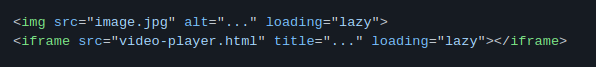
\includegraphics[scale=0.5]{chapitre2/wdd4/fig/c1.png}
\end{figure}
\end{block}

\begin{block}{Utiliser le rechargement partiel d'une zone de contenu}
Procéder à un rechargement uniquement des changements et non pas de toute la page. 
\end{block}


\end{frame}


\begin{frame}{Bonnes pratiques dans le numérique}{Conseils 36-38/115}
\begin{block}{Éviter les animations JavaScript / CSS}
Les animations JavaScript/CSS peuvent être très coûteuses en termes de cycles CPU et de consommation mémoire
\end{block}

\begin{block}{N'utilisez que les portions indispensables des librairies JavaScript et frameworks CSS}

Se passer des bibliothèques JavaScript ou n’en conserver que les portions réellement utilisées.
Utiliser un bundler (ex: Webpack) permet de faire facilement du tree shaking, soit d'éliminer du code "mort" donc non utilisé
\end{block}

\begin{block}{Ne pas faire de modification du DOM lorsqu’on le traverse}

\begin{minipage}[b]{0.35\linewidth}
Modifier le DOM (Document Object Model) est gachis en cycles CPU
\end{minipage}\hfill
\begin{minipage}[b]{0.65\linewidth}
\begin{figure}
    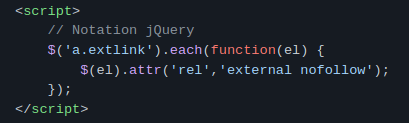
\includegraphics[scale=0.4]{chapitre2/wdd4/fig/c2.png}
\end{figure}
\end{minipage}\hfill
\end{block}
\end{frame}


\begin{frame}{Bonnes pratiques dans le numérique}{Conseils 39-40/115}
\begin{block}{Rendre les éléments du DOM invisibles lors de leur modification}

Lorsqu’un élément du DOM doit être modifié, il est plus économe de :
\begin{itemize}
    \item rendre l’élément invisible (passer la propriété display à none) (1 reflow)
    \item modifier toutes les propriétés de l’élément et rendre l’élément à nou-veau visible (1 reflow).
\end{itemize}
   \begin{figure}
    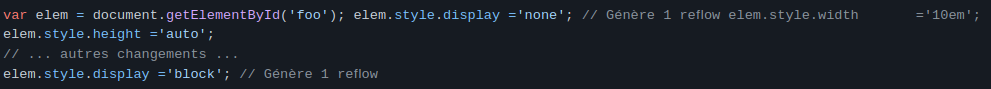
\includegraphics[scale=0.3]{chapitre2/wdd4/fig/c3.png}
\end{figure} 
\end{block}

\begin{block}{Réduire au maximum le repaint (appearence) et le reflow (layout)}

\begin{itemize}
    \item Ne pas modifier les propriétés stylistiques d’un élément
    \item Limiter les changements de propriétés de position, de dimension, de type de positionnement, de contenu
\end{itemize}

\end{block}


\end{frame}

\begin{frame}{Bonnes pratiques dans le numérique}{Conseil 41/115}
\begin{block}{Utiliser la délégation d'évènements}
La délégation d’événements permet de ne pas surcharger la mémoire du navigateur (un seul écouteur pour plusieurs éléments du DOM)

   \begin{figure}
    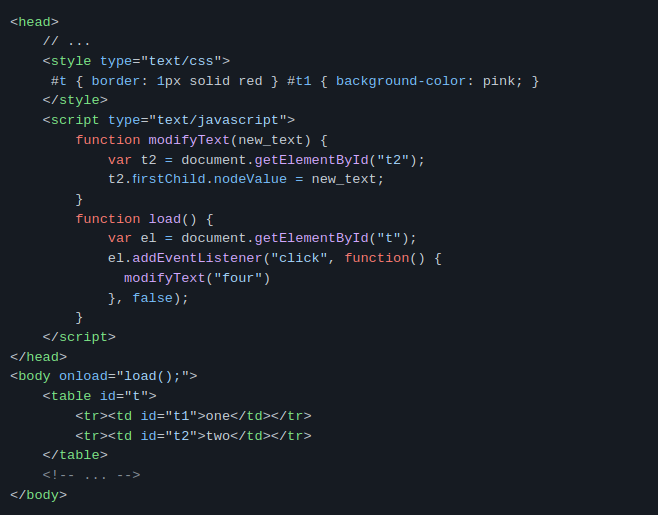
\includegraphics[scale=0.3]{chapitre2/wdd4/fig/c4.png}
\end{figure} 
\end{block}
\end{frame}




\begin{frame}{Bonnes pratiques dans le numérique}{Conseil 42-44/115}
\begin{block}{Modifier plusieurs propriétés CSS en 1 seule fois}
Ne pas modifier des propriétés une à une (plutôt modifier les classes CSS).
\end{block}
\begin{block}{Valider votre code avec un Linter}
\begin{itemize}
    \item  ESLint pour le code JavaScript
    \item Stylelint pour vs feuilles de styles
\end{itemize}
\end{block}

\begin{block}{Mettre en cache les objets souvent accédés en JavaScript}
L’accès au DOM est coûteux en cycles CPU.
\begin{figure}
    \centering
    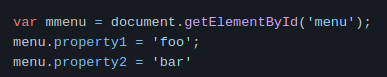
\includegraphics[scale=0.35]{chapitre2/wdd4/fig/c6.png}
\end{figure}
\begin{figure}
    \centering
    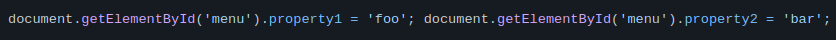
\includegraphics[scale=0.35]{chapitre2/wdd4/fig/c7.png}
\end{figure}
\end{block}


\end{frame}


\begin{frame}{Pause débunkage }{Zones invivables}
\begin{figure}
    \centering
    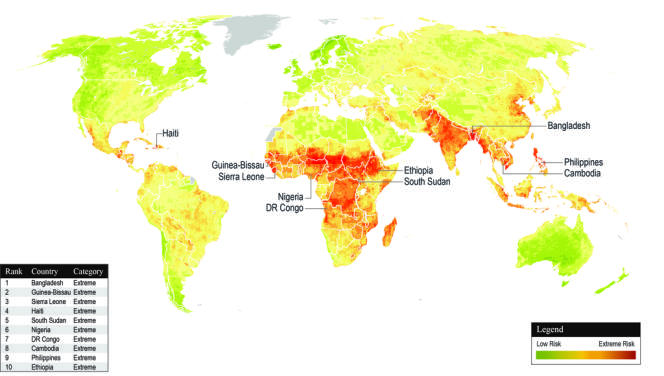
\includegraphics[scale=2]{chapitre2/wdd4/fig/climat.jpg}
\end{figure}
\end{frame}